\chapter{Energie und der Hamiltonian}

\lectureoverview{Zunächst präzisieren wir die Bedeutung einer aktiven Symmetrie und wiederholen, wie Translationen und Drehungen Impuls und Drehimpuls hervorbringen. Die noch fehlende Erhaltungsgröße ist die Energie. Die zugehörige Symmetrie ist die Translation in der Zeit; die erhaltene Größe ist der Hamiltonian \(H=\sum_i p_i\dot q_i-L\). Die Herleitung zeigt außerdem genau, wie explizite Zeitabhängigkeit Energie zwischen einem ausgewählten Teilsystem und seiner Umgebung überträgt.}

\section{Fragen vor der formalen Herleitung}

Wir nähern uns dem absoluten Minimum an klassischer Mechanik, das für die folgenden Themen erforderlich ist, auch wenn es noch viel mehr Mechanik gibt, die zu lernen sich lohnt. Noch vor Beginn der eigentlichen Herleitung kamen zwei Fragen auf.

\begin{classroomqa}\audiencequestion{Welche Bücher eignen sich im Anschluss an diesen Einführungskurs?\lecturetimestamp{00:00:36--00:02:13}}\lecturerresponse{Das etablierte fortgeschrittene Nachschlagewerk ist Herbert Goldsteins \emph{Classical Mechanics}. Auch Cornelius Lanczos’ Buch über die Variationsprinzipien der Mechanik ist eine einschlägige Quelle. Eine Leseliste für den Kurs ist hilfreicher, als so zu tun, als könne eine einzelne Lehrperson einen Überblick über alle verfügbaren Texte geben.}\end{classroomqa}

Die zweite Frage hält einen Moment in der Geschichte einer damals noch ungeklärten Messung fest. 2011 hatte das OPERA-Experiment eine scheinbar frühe Ankunft von Neutrinos gemeldet, die vom CERN zum Gran-Sasso-Labor geschickt worden waren. Die gemeldete Abweichung war kürzer als der Protonenpuls, mit dem die Neutrinos erzeugt wurden. Deshalb beruhte die Zeitmessung darauf, Pulsprofile miteinander zu vergleichen, statt ein einzelnes Neutrino beim Aussenden zu markieren und dasselbe Teilchen beim Nachweis wiederzuerkennen.

\begin{classroomqa}\audiencequestion{War das scheinbare Ergebnis, dass sich Neutrinos schneller als Licht bewegen, inzwischen geklärt?\lecturetimestamp{00:02:30--00:09:03}}\lecturerresponse{Damals ließ sich noch keine Schlussfolgerung rechtfertigen. Pulsform des Strahls, Erwärmung des Targets und Synchronisation mussten technisch genau geprüft werden. Ein spekulativer Vorschlag bezog die Bewegung eines GPS-Satelliten ein: Im Bezugssystem des Satelliten bewegen sich Quelle und Detektor, während die Zeitsignale unterwegs sind; dadurch entstehen Korrekturen in der Größenordnung einiger zehn Nanosekunden. Als Abschätzung der Größenordnung war das interessant, wurde aber nicht als glaubwürdige Erklärung des Experiments präsentiert. Die gewöhnliche Lorentz-Kontraktion bei der betreffenden Geschwindigkeit war viel zu klein, um den gemeldeten Effekt zu erklären. Die angemessene Reaktion war, die experimentelle Analyse abzuwarten.}\end{classroomqa}

\begin{figure}[htbp]\centering
  \includegraphics[width=0.78\textwidth]{lecture_05_figure_07.png}\caption{Skizze der Zeitmessung im Bezugssystem des Satelliten, die im Zusammenhang mit der historischen Frage zur Neutrinomessung besprochen wurde.}\lectureframe{00:06:30}\end{figure}

Die Diskussion der Zeitmessung wird für die folgende Mechanik nicht benötigt. Sie erinnert jedoch daran, dass eine plausible Abschätzung der Größenordnung noch keine gesicherte experimentelle Erklärung ist.

\section{Aktive Symmetrie und die Wahl des Systems}

Kehren wir zu dem Punkt zurück, der in der vorangegangenen Diskussion noch zu unklar geblieben ist: Was genau ist eine Symmetrie? Betrachten wir ein Teilchen auf einer Geraden und die Vorschrift \begin{equation}
  x\longrightarrow x+1.
  \label{eq:l5-shift-one}
\end{equation}. Es gibt zwei Möglichkeiten, sie zu verstehen. Eine \emph{passive} Transformation benennt die Punkte der Geraden um. Ein Punkt, der zuvor \(x=0\) hieß, kann nun \(x'=1\) heißen; das Teilchen hat sich dabei aber nicht bewegt. Eine \emph{aktive} Transformation lässt die Bezeichnungen unverändert und bewegt das Teilchen selbst von \(x\) nach \(x+1\). Nur die zweite Operation verändert seine Position relativ zu einem äußeren Potential.

\begin{figure}[htbp]\centering
  \includegraphics[width=0.82\textwidth]{lecture_05_figure_08.png}\caption{\(x\mapsto x+1\), die festgehaltene Koordinatengerade und ein äußeres Potential machen den Unterschied zwischen aktiver Bewegung und passiver Umbenennung deutlich.}\lectureframe{00:11:20}\end{figure}

\begin{classroomqa}\audiencequestion{Wird die Quelle des Potentials aus dem System ausgeschlossen, wenn eine Bewegung des Teilchens seine potenzielle Energie ändert?\lecturetimestamp{00:12:19--00:14:18}}\lecturerresponse{Genau. Wenn man das System als ``Teilchen in einem Potential'' bezeichnet, teilt man die Welt in das Teilchen und eine schwere Umgebung auf, etwa die Erde, die \(V(x)\) erzeugt. Die Erde erfährt zwar einen Rückstoß, doch aufgrund ihrer enormen Masse ist dieser in dieser Näherung vernachlässigbar. Eine Bewegung des Teilchens relativ zur ruhenden Erde kann \(V\) ändern; eine gemeinsame Translation von Teilchen und Erde würde das nicht tun.}\end{classroomqa}

\begin{classroomqa}\audiencequestion{Wurden im früheren Beispiel mit der Drehung auch die Geschwindigkeiten verändert, oder nur die Positionen?\lecturetimestamp{00:14:26--00:15:29}}\lecturerresponse{Ja. Eine starre aktive Drehung wirkt auf die gesamte Bewegungsgeschichte, nicht nur auf eine momentane Position. Sowohl Positionen als auch Geschwindigkeitsvektoren werden gedreht. Eine dagegen zu jedem Zeitpunkt ausgeführte konstante Translation ändert \(x\), lässt aber \(\dot x\) unverändert.}\end{classroomqa}

Der Unterschied zwischen System und Umgebung wird noch zweimal eine Rolle spielen: wenn ein zeitabhängiger Apparat Energie mit einem Teilsystem austauscht und wenn makroskopische Reibung Energie in unbeobachtbarer mikroskopischer Bewegung verbirgt.

\section{Infinitesimale Bewegungen im Konfigurationsraum}

Die Konfiguration eines allgemeinen mechanischen Systems ist ein Punkt im Raum der verallgemeinerten Koordinaten \(q_i\). Eine aktive infinitesimale Transformation bewegt jede mögliche Konfiguration in eine benachbarte. Wir schreiben \begin{equation}
  \delta q_i=\epsilon f_i(q),
  \label{eq:l5-general-transformation}
\end{equation}, wobei die Funktionen \(f_i\) ein festes Verschiebungsfeld im Konfigurationsraum festlegen. Sie können von sämtlichen Koordinaten abhängen; einige können auch verschwinden. Der gemeinsame Faktor \(\epsilon\) ist klein; er trennt die Schrittweite von der Form der Transformation.

\begin{figure}[htbp]\centering
  \includegraphics[width=0.75\textwidth]{lecture_05_figure_09.png}\caption{Ein Verschiebungsvektor, der jedem Punkt des Konfigurationsraums zugeordnet ist.}\lectureframe{00:16:50}\end{figure}

\begin{figure}[htbp]\centering
  \includegraphics[width=0.80\textwidth]{lecture_05_figure_10.png}\caption{Die koordinatenabhängige infinitesimale Transformation \(\delta q_i=\epsilon f_i(q)\).}\lectureframe{00:18:00}\end{figure}

Die Vorschrift selbst hängt nicht explizit von der Zeit ab. Ihre Wirkung auf die Geschwindigkeiten ist daher \begin{equation}
  \delta\dot q_i=\frac{d}{dt}(\delta q_i)
  =\epsilon\sum_j\frac{\partial f_i}{\partial q_j}\dot q_j.
  \label{eq:l5-velocity-variation}
\end{equation}. Bei einer Translation gilt \(f_x=1\), also \(\delta\dot x=0\). Bei einer Drehung hängt \(f_i\) von der Position ab, und die Geschwindigkeit ändert sich.

\begin{classroomqa}\audiencequestion{Ist der letzte kleine Faktor in \(\delta q_i=\epsilon f_i(q)\) an jedem Punkt dieselbe Konstante?\lecturetimestamp{00:19:58--00:20:51}}\lecturerresponse{Ja. Die einzelne Konstante \(\epsilon\) dient als Hilfsgröße, durch die alle Koordinatenänderungen von derselben kleinen Größe erster Ordnung abhängen. Die räumliche Abhängigkeit steckt in den Funktionen \(f_i(q)\), nicht in \(\epsilon\); die Funktionen müssen selbst nicht klein sein.}\end{classroomqa}

\section{Wann ist die Transformation eine Symmetrie?}

Eine aktive Transformation ändert im Allgemeinen die potenzielle Energie. Sie kann auch die kinetische Energie ändern. In krummlinigen Koordinaten hat der kinetische Term die Form \begin{equation}
  T=\frac12\sum_{i,j}g_{ij}(q)\dot q_i\dot q_j,
  \label{eq:l5-kinetic-metric}
\end{equation}, sodass sich seine Koeffizienten bei einer Bewegung im Konfigurationsraum ändern können. Der bekannte Term \(r^2\dot\theta^2\) in Polarkoordinaten ist das einfachste Beispiel dafür.

Eine Transformation ist hier eine Symmetrie, wenn sich die \emph{gesamte} Lagrangefunktion in erster Ordnung nicht ändert: \begin{equation}
  \delta L=O(\epsilon^2),
  \label{eq:l5-symmetry-condition}
\end{equation}. Dies muss an jedem Punkt des Konfigurationsraums gelten, nicht nur für die Konfiguration, die eine bestimmte Lösung gerade einnimmt.

Zum Beispiel gilt für \(x\mapsto x+\epsilon\): \begin{equation}
  \delta V=\frac{\partial V}{\partial x}\epsilon.
  \label{eq:l5-potential-variation}
\end{equation}. Verschwindet dieser Ausdruck für jedes mögliche \(x\), dann gilt \(\partial V/\partial x=0\): Das Potential ist unabhängig von \(x\). Bleibt es unter Translationen in jeder räumlichen Richtung unverändert, ist es konstant.

\begin{figure}[htbp]\centering
  \includegraphics[width=0.80\textwidth]{lecture_05_figure_11.png}\caption{\(x\)-Translation, geprüft an einem Potential \(V(y)\), das unabhängig von \(x\) ist.}\lectureframe{00:23:40}\end{figure}

Für eine glatte einparametrige Familie lässt sich aus dem Verschwinden der Änderung erster Ordnung an jedem Punkt durch Verkettung infinitesimaler Schritte eine endliche Symmetrie zusammensetzen.

\begin{classroomqa}\audiencequestion{Müssen kinetische und potenzielle Energie jeweils für sich erhalten bleiben?\lecturetimestamp{00:24:44--00:25:33}}\lecturerresponse{Nein. Invariant sein muss nur die gesamte Lagrangefunktion. Manche Lagrangefunktionen enthalten gemischte Terme aus Koordinaten-- und Geschwindigkeiten und lassen sich nicht sinnvoll in \(T\) und \(V\) aufteilen. Eine getrennte Invarianz ist dann womöglich gar keine sinnvolle Fragestellung.}\end{classroomqa}

\begin{classroomqa}\audiencequestion{Bedeutet ``keine Änderung'' eine exakt verschwindende Änderung oder nur eine, die klein genug ist, um vernachlässigt zu werden?\lecturetimestamp{00:25:34--00:28:59}}\lecturerresponse{Bei einer infinitesimalen Transformation bedeutet es, dass kein Term proportional zu \(\epsilon\) auftritt. Terme der Ordnung \(\epsilon^2\) werden in der lokalen Rechnung verworfen. Da die Bedingung erster Ordnung entlang der gesamten einparametrigen Bahn gilt, führt die Wiederholung des lokalen Schritts zur endlichen Invarianz.}\end{classroomqa}

\section{Impuls und Drehimpuls wiedergewonnen}

Für die hier betrachteten exakten, zeitunabhängigen Punktsymmetrien lautet das zuvor bewiesene Ergebnis \begin{equation}
  Q=\sum_i p_i f_i(q),
  \qquad
  p_i=\frac{\partial L}{\partial\dot q_i},
  \qquad
  \dot Q=0.
  \label{eq:l5-noether-charge}
\end{equation}. Der Faktor \(\epsilon\) gehört nicht zu \(Q\); er gibt lediglich an, wie weit wir uns entlang der Symmetriebahn bewegen.

\begin{figure}[htbp]\centering
  \includegraphics[width=0.82\textwidth]{lecture_05_figure_12.png}\caption{Die allgemeine infinitesimale Verschiebung und die zugehörige erhaltene Noether-Ladung.}\lectureframe{00:30:00}\end{figure}

Für eine Translation in \(x\) gilt \(f_x=1\) und \(Q=p_x\). Volle Translationsinvarianz führt zur Erhaltung aller drei Impulskomponenten. Bei vielen wechselwirkenden Teilchen werden alle Teilchen gemeinsam durch die Symmetrie translationiert. Daher ist \begin{equation}
  \mathbf P=\sum_a\mathbf p_a
  \label{eq:l5-total-momentum}
\end{equation} erhalten, wenn die Wechselwirkungen nur von den Relativpositionen abhängen. Ein Teilchen relativ zum Rest zu bewegen, ist keine Symmetrie.

\begin{figure}[htbp]\centering
  \includegraphics[width=0.80\textwidth]{lecture_05_figure_13.png}\caption{Eine gemeinsame Translation führt komponentenweise zur Erhaltung des Gesamtimpulses.}\lectureframe{00:32:50}\end{figure}

Für eine infinitesimale Drehung in der \(x\)-\(y\)-Ebene wählen wir die Orientierung \begin{equation}
  \delta x=-y\epsilon,
  \qquad
  \delta y=x\epsilon.
  \label{eq:l5-planar-rotation}
\end{equation}. Der Abstand vom Ursprung bleibt erhalten, denn \begin{equation}
  \delta(x^2+y^2)
  =2x\delta x+2y\delta y=0.
  \label{eq:l5-radius-invariance}
\end{equation}.

\begin{figure}[htbp]\centering
  \includegraphics[width=0.76\textwidth]{lecture_05_figure_14.png}\caption{Geometrie und Koordinatenformel einer infinitesimalen Drehung in der Ebene.}\lectureframe{00:35:05}\end{figure}

Durch Differenzieren von Gl.~\eqref{eq:l5-planar-rotation} zeigt sich, dass auch die Geschwindigkeiten gedreht werden. Daher ist \(\dot x^2+\dot y^2\) invariant, und ein Zentralpotential \(V(\sqrt{x^2+y^2})\) lässt die vollständige Lagrangefunktion unverändert. Die zugehörige Ladung ist \begin{equation}
  Q=-yp_x+xp_y=(\mathbf r\times\mathbf p)_z.
  \label{eq:l5-angular-charge}
\end{equation}.

\begin{figure}[htbp]\centering
  \includegraphics[width=0.76\textwidth]{lecture_05_figure_15.png}\caption{Die Noether-Ladung der Drehung, die \(z\)-Komponente des Drehimpulses.}\lectureframe{00:38:50}\end{figure}

Drehungen in den anderen Koordinatenebenen liefern die übrigen Komponenten. Für viele Teilchen ist der erhaltene Vektor \begin{equation}
  \mathbf J=\sum_a\mathbf r_a\times\mathbf p_a.
  \label{eq:l5-total-angular-momentum}
\end{equation}. Ein Planet im Zentralpotential eines Sterns ist das grundlegende Beispiel: Die Invarianz unter allen Drehungen impliziert die Erhaltung aller Drehimpulskomponenten.

\begin{classroomqa}\audiencequestion{Was geschieht an einer scharfen Spitze, wenn sich die Ableitung auf der einen Seite von der auf der anderen Seite unterscheidet?\lecturetimestamp{00:42:25--00:44:21}}\lecturerresponse{Das ist ein berechtigter Vorbehalt. Die vorliegende Herleitung setzt differenzierbare Funktionen mit eindeutigen Ableitungen voraus. Ein instabiles Gleichgewicht, etwa ein Körper, der auf einem glatten Maximum im Gleichgewicht gehalten wird, ist für sich genommen kein Problem: Die Ableitung existiert dort und verschwindet. Eine echte Spitze erfordert eine angepasste Behandlung.}\end{classroomqa}

\begin{classroomqa}\audiencequestion{Wenn der Transformationsparameter zeitunabhängig ist, warum ändert eine Drehung dann die Geschwindigkeiten?\lecturetimestamp{00:44:23--00:45:23}}\lecturerresponse{Der Parameter ist konstant, aber das Verschiebungsfeld hängt von den Koordinaten ab. Die allgemeine Vorschrift lautet \(\delta\dot q_i=d(\delta q_i)/dt\). Bei einer Translation ist \(\delta x\) konstant, wohingegen bei einer Drehung \(\delta x=-y\epsilon\) gilt und daher \(\delta\dot x=-\dot y\epsilon\).}\end{classroomqa}

\section{Über die elementare Form „kinetische minus potenzielle Energie“ hinaus}

Für gewöhnliche nichtrelativistische Teilchen in kartesischen Koordinaten und ohne Magnetfelder gilt \(L=T-V\). Allgemeinere Koordinaten führen zur quadratischen Form aus Gl.~\eqref{eq:l5-kinetic-metric}. Ein Magnetfeld bringt einen linearen Term in der Geschwindigkeit mit sich, schematisch \(\mathbf A(q)\cdot\dot{\mathbf q}\), der Koordinaten und Geschwindigkeiten miteinander verknüpft. In einem solchen Fall ist es besser, \(L(q,\dot q,t)\) als eine einzige Funktion zu behandeln, statt jeden Term gewaltsam einer der üblichen Kategorien kinetische oder potenzielle Energie zuzuordnen.

\begin{figure}[htbp]\centering
  \includegraphics[width=0.80\textwidth]{lecture_05_figure_16.png}\caption{Ein allgemeiner koordinatenabhängiger quadratischer kinetischer Term neben einem nur von den Koordinaten abhängigen Potential.}\lectureframe{00:47:20}\end{figure}

\begin{classroomqa}\audiencequestion{Warum lässt sich eine Lagrangefunktion möglicherweise nicht sauber in kinetische und potenzielle Energie zerlegen, und ist sie trotzdem als \(T-V\) definiert?\lecturetimestamp{00:45:26--00:48:13}}\lecturerresponse{Das kann an krummlinigen Koordinaten oder an echten geschwindigkeitsabhängigen Wechselwirkungen wie dem Magnetismus liegen. Nur wenn die Lagrangefunktion aus einer quadratischen Form der Geschwindigkeiten minus einer ausschließlich koordinatenabhängigen Funktion besteht, bezeichnen wir diese Teile als \(T\) und \(V\). Andernfalls bleibt die Lagrangefunktion eine vollkommen zulässige Funktion von \(q\) und \(\dot q\), aber die Aufteilung ist nicht hilfreich. Die korrekte allgemeine Definition der Energie wird sich aus dem Hamiltonian ergeben.}\end{classroomqa}

\begin{classroomqa}\audiencequestion{War das Beispiel mit der hängenden Kette aus der ersten Sitzung eine Anwendung des Prinzips der kleinsten Wirkung?\lecturetimestamp{00:48:15--00:49:45}}\lecturerresponse{Es war ein Gleichgewichtsproblem, das dem Prinzip der kleinsten Energie folgt, und keine durch stationäre Wirkung ausgewählte Bewegungsgeschichte. Für eine statische Lösung eines gewöhnlichen Systems der Form \(T-V\) gilt \(\dot p_i=0\), und die Euler---Lagrange-Gleichung reduziert sich auf \(\partial V/\partial q_i=0\), die Bedingung dafür, dass das Potential einen stationären Punkt hat.}\end{classroomqa}

Impuls und Drehimpuls sind nun mit räumlichen Symmetrien verknüpft. Die auffällig fehlende Größe ist die Energie.

\section{Translationsinvarianz in der Zeit}

Stellen wir uns ein Experiment vor, das bei \(t_0\) beginnt, bei \(t_1\) endet und ein Ergebnis liefert. Wiederholen wir dieselbe Präparation später, mit Beginn bei \(t_0+\Delta t\) und Ende bei \(t_1+\Delta t\). Bleibt das Ergebnis unverändert, ist das System unter einer aktiven Translation in der Zeit invariant.

\begin{figure}[htbp]\centering
  \includegraphics[width=0.82\textwidth]{lecture_05_figure_17.png}\caption{Ein Experiment und seine zeitlich verschobene Kopie im Konfigurationsraum der Bewegungsgeschichte.}\lectureframe{00:52:45}\end{figure}

Ein geladenes Teilchen zwischen Kondensatorplatten veranschaulicht das Versagen dieser Symmetrie. Bei fester Ladung auf den Platten lässt sich dasselbe Experiment zu jedem beliebigen Zeitpunkt durchführen. Lädt ein äußerer Generator die Platten fortlaufend auf, sieht das Teilchen je nach Freisetzungszeit ein anderes elektrisches Feld. Das Teilchen ist dann ein explizit angetriebenes Teilsystem.

\begin{figure}[htbp]\centering
  \includegraphics[width=0.82\textwidth]{lecture_05_figure_18.png}\caption{Feste und sich äußerlich verändernde Kondensatorplatten im Vergleich, neben der Darstellung der Zeittranslation.}\lectureframe{00:54:45}\end{figure}

Derselbe Punkt zeigt sich bei einem Oszillator: \begin{equation}
  L=\frac12m\dot x^2-\frac12k(t)x^2.
  \label{eq:l5-driven-oscillator}
\end{equation}. Ein äußeres elektrisches oder magnetisches Feld könnte das Material langsam verändern und damit auch seine effektive Federkonstante. Wenn \(k\) variiert, ändert sich das Ergebnis, sobald man das Oszillatorexperiment zeitlich verschiebt.

\begin{figure}[htbp]\centering
  \includegraphics[width=0.78\textwidth]{lecture_05_figure_19.png}\caption{Kinetische und potenzielle Terme des Oszillators bei der Diskussion einer zeitabhängigen Federkonstante.}\lectureframe{00:56:45}\end{figure}

Nimmt man den Apparat, der \(k\) verändert, in das System auf, lässt sich das gesamte abgeschlossene Experiment wieder zeitlich verschieben, und seine Gesamtenergie bleibt erhalten. Die scheinbare Nichterhaltung ist ein Energieaustausch über eine von uns gewählte Systemgrenze.

In der Pause wurde der kleine Transformationsparameter in \(\epsilon\) umbenannt, um den optisch verwirrenden Ausdruck \(\delta x=\delta\) zu vermeiden. Außerdem wurde für die gemeinsame Leseliste ein Buch über Emmy Noether empfohlen.

\begin{classroomqa}\audiencequestion{Wenn die Lagrangefunktion nicht als \(T-V\) vorgegeben ist, woher stammt sie dann?\lecturetimestamp{01:00:17--01:02:24}}\lecturerresponse{Sie lässt sich aus Experimenten erschließen, aus bekannten Bewegungsgleichungen rekonstruieren, aufgrund von Symmetrie und anderen theoretischen Prinzipien vermuten oder durch Ausprobieren finden. Sobald \(L(q,\dot q,t)\) gegeben ist, führt die Euler---Lagrange-Rechnung zu den Bewegungsgleichungen. Die formale Herleitung setzt nicht voraus, dass wir zuerst den Ursprung der Lagrangefunktion klären.}\end{classroomqa}

Die operationale Prüfung auf Zeittranslationsinvarianz ist nun unmittelbar. Reichen die Kenntnis von \(q\) und \(\dot q\) aus, um \(L\) zu bestimmen, ohne zusätzlich die Uhrzeit kennen zu müssen, dann gilt \begin{equation}
  \frac{\partial L}{\partial t}=0.
  \label{eq:l5-no-explicit-time}
\end{equation}. Das besagt nicht, dass \(L(q(t),\dot q(t))\) während einer Bewegung konstant ist. Es besagt nur, dass es keine Zeitabhängigkeit gibt, die über diejenige hinausgeht, die durch die sich entwickelnden Koordinaten und Geschwindigkeiten vermittelt wird.

Ein rotierendes schweres Hantelmodell ist ein weiteres Beispiel für ein angetriebenes System. Erzeugt seine vorgegebene Bewegung für ein leichtes Probeteilchen ein zeitlich veränderliches Gravitationspotential, so hängt die Lagrangefunktion des Probeteilchens explizit von der Zeit ab. Behandelte man die Hantel stattdessen dynamisch, würde man das System erweitern und diese äußere Zeitabhängigkeit beseitigen.

\begin{figure}[htbp]\centering
  \includegraphics[width=0.80\textwidth]{lecture_05_figure_20.png}\caption{Eine vorgegebene rotierende Hantel wirkt als zeitabhängige äußere Quelle auf ein leichteres Teilchen.}\lectureframe{01:06:25}\end{figure}

\section{Herleitung des Hamiltonians}

Nehmen wir an, wir wüssten nichts über die Formel für die Energie und vermuteten, dass vielleicht die Lagrangefunktion selbst erhalten ist. Das lässt sich direkt prüfen, indem man sie entlang einer tatsächlichen Bahn ableitet. Beginnen wir der Einfachheit halber ohne explizite Zeitabhängigkeit: \begin{equation}
  \frac{dL}{dt}
  =\sum_i\left(
    \frac{\partial L}{\partial q_i}\dot q_i
    +\frac{\partial L}{\partial\dot q_i}\ddot q_i
  \right).
  \label{eq:l5-chain-rule-no-time}
\end{equation}

\begin{figure}[htbp]\centering
  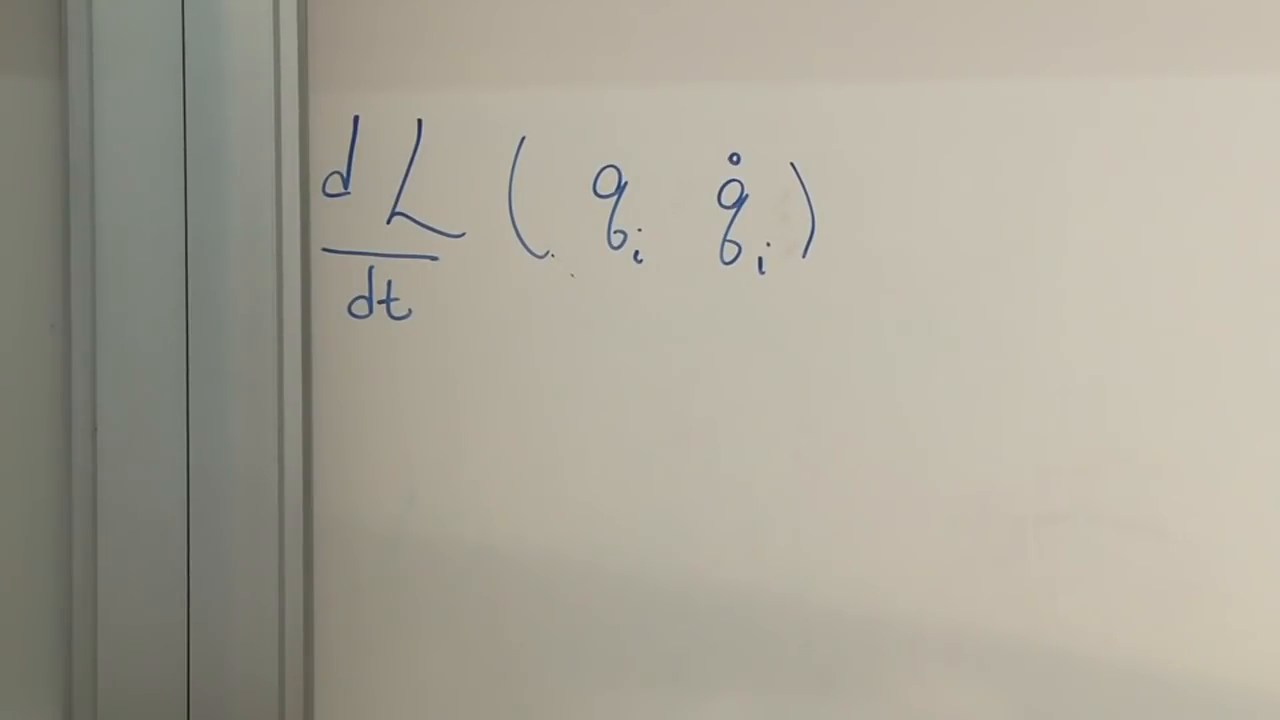
\includegraphics[width=0.72\textwidth]{lecture_05_figure_02.png}\caption{Beginn der Ableitung von \(L(q_i,\dot q_i)\) entlang der Bahn.}\lectureframe{01:08:51}\end{figure}

\begin{classroomqa}\audiencequestion{Fehlt in dem Ausdruck für die Kettenregel eine Summe?\lecturetimestamp{01:10:39--01:11:05}}\lecturerresponse{Ja. Jede Koordinate und jede Geschwindigkeit kann die Lagrangefunktion ändern, also werden beide Terme über \(i\) summiert.}\end{classroomqa}

Verwenden wir den kanonischen Impuls und die Euler---Lagrange-Gleichung: \begin{equation}
  p_i=\frac{\partial L}{\partial\dot q_i},
  \qquad
  \dot p_i=\frac{\partial L}{\partial q_i}.
  \label{eq:l5-p-and-pdot}
\end{equation}. Dann wird Gl.~\eqref{eq:l5-chain-rule-no-time} zu \begin{align}
  \frac{dL}{dt}
  &=\sum_i(\dot p_i\dot q_i+p_i\ddot q_i)
  \notag\\
  &=\frac{d}{dt}\sum_i p_i\dot q_i.
  \label{eq:l5-product-rule}
\end{align}. Der ``Trick'' besteht lediglich in der Produktregel.

\begin{figure}[htbp]\centering
  \includegraphics[width=0.84\textwidth]{lecture_05_figure_21.png}\caption{Die Kettenregel wird mithilfe der Bewegungsgleichungen zur Ableitung von \(\sum_i p_i\dot q_i\).}\lectureframe{01:13:45}\end{figure}

\begin{classroomqa}\audiencequestion{Muss im letzten Produkt \(q_i\) einmal oder zweimal punktiert sein?\lecturetimestamp{01:14:31--01:15:32}}\lecturerresponse{Im Produkt steht \(p_i\dot q_i\) mit einem Punkt. Beim Ableiten des Produkts ergibt sich \(\dot p_i\dot q_i+p_i\ddot q_i\); daher treten im ausmultiplizierten zweiten Term zwei Punkte auf.}\end{classroomqa}

Durch Subtraktion der beiden Ableitungen erhält man eine erhaltene Kombination. Der historischen Konvention folgend wählen wir ihr Negatives und nennen es den Hamiltonian: \begin{equation}
  H=\sum_i p_i\dot q_i-L.
  \label{eq:l5-hamiltonian-definition}
\end{equation}

\begin{figure}[htbp]\centering
  \includegraphics[width=0.80\textwidth]{lecture_05_figure_22.png}\caption{Die erhaltene Kombination \(L-\sum_i p_i\dot q_i=-H\) und die Definition des Hamiltonians.}\lectureframe{01:18:05}\end{figure}

Für ein Teilchen in einem Potential gilt \begin{equation}
  L=\frac12m\dot x^2-V(x),
  \qquad p=m\dot x.
  \label{eq:l5-particle-lagrangian}
\end{equation}. Daher \begin{align}
  H&=p\dot x-L
  \notag\\
   &=m\dot x^2-\left(\frac12m\dot x^2-V(x)\right)
  \notag\\
   &=\frac12m\dot x^2+V(x)=T+V.
  \label{eq:l5-particle-energy}
\end{align}.

\begin{figure}[htbp]\centering
  \includegraphics[width=0.86\textwidth]{lecture_05_figure_23.png}\caption{Der Hamiltonian eines Teilchens in einem Potential reduziert sich auf die bekannte Summe aus kinetischer und potenzieller Energie.}\lectureframe{01:20:50}\end{figure}

Bei der Herleitung wurde keine bestimmte Form von \(L\) vorausgesetzt. Daher ist Gl.~\eqref{eq:l5-hamiltonian-definition}, nicht \(T+V\), in diesem Formalismus die allgemeine Definition der Energie.

\section{Explizite Zeitabhängigkeit und Energieaustausch}

Nehmen wir die explizite Zeitabhängigkeit wieder in die Kettenregel auf: \begin{equation}
  \frac{dL}{dt}
  =\sum_i\left(
    \frac{\partial L}{\partial q_i}\dot q_i
    +\frac{\partial L}{\partial\dot q_i}\ddot q_i
  \right)
  +\frac{\partial L}{\partial t}.
  \label{eq:l5-full-chain-rule}
\end{equation}. Die linke Seite ist die totale Ableitung entlang der Bewegung. Bei der letzten partiellen Ableitung werden \(q\) und \(\dot q\) konstant gehalten; sie berücksichtigt nur Parameter, die sich aufgrund äußerer Einflüsse ändern. Wiederholen wir denselben Schritt mit der Produktregel, ergibt sich \begin{equation}
  \boxed{\frac{dH}{dt}=-\frac{\partial L}{\partial t}}.
  \label{eq:l5-hamiltonian-time}
\end{equation}.

\begin{figure}[htbp]\centering
  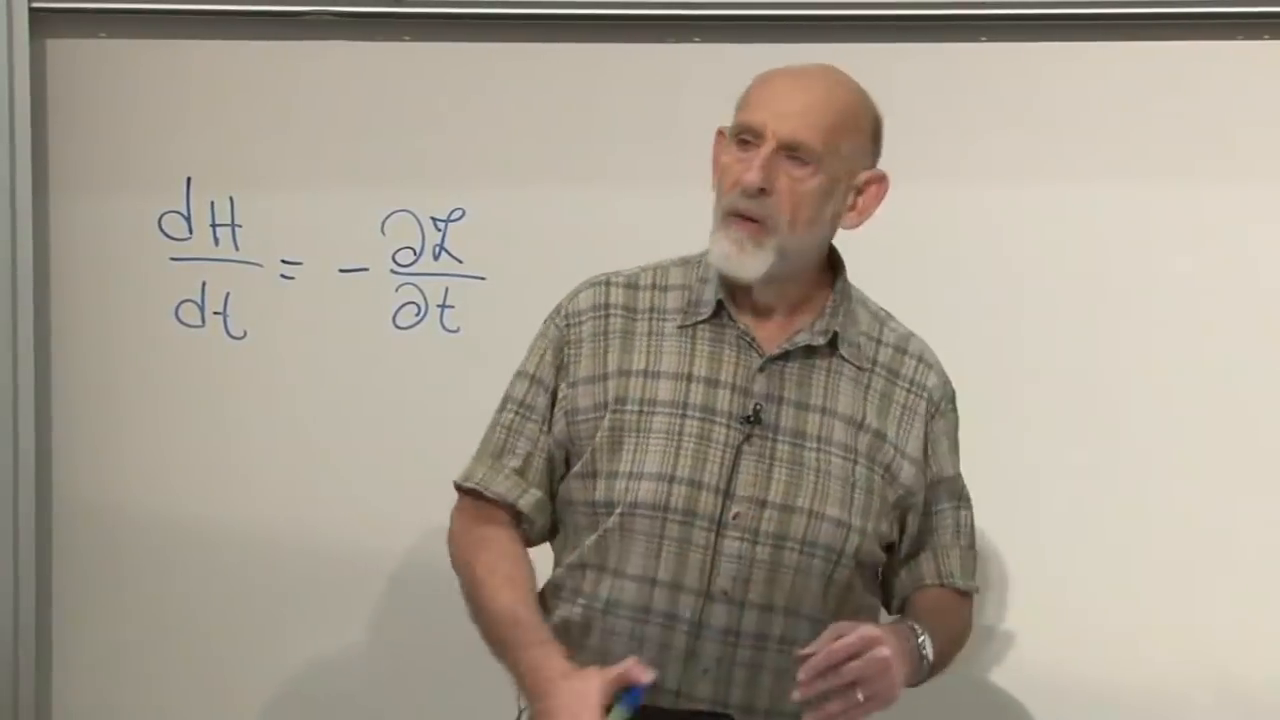
\includegraphics[width=0.70\textwidth]{lecture_05_figure_04.png}\caption{Der Hamiltonian ändert sich nur aufgrund der expliziten Zeitabhängigkeit der Lagrangefunktion.}\lectureframe{01:37:22}\end{figure}

Für den angetriebenen Oszillator aus Gl.~\eqref{eq:l5-driven-oscillator} gilt \begin{equation}
  \frac{\partial L}{\partial t}
  =-\frac12\dot k(t)x^2,
  \qquad
  \dot H=\frac12\dot k(t)x^2.
  \label{eq:l5-driven-energy-rate}
\end{equation}. Bei \(x=0\) verschwindet die momentane Änderungsrate; außerhalb des Ursprungs leistet die Änderung der Federkonstante Arbeit mit einer Rate proportional zu \(x^2\dot k\).

\begin{classroomqa}\audiencequestion{Wenn die Energie nicht erhalten ist, ist ihre Definition dann die Zeitableitung des Hamiltonians?\lecturetimestamp{01:27:11--01:28:04}}\lecturerresponse{Nein. Die Energie ist \(H\). Ihre Ableitung sagt uns, wie sich diese Energie ändert. Hat die Lagrangefunktion die vertraute Form, gilt \(H=T+V\); andernfalls liefert Gl.~\eqref{eq:l5-hamiltonian-definition} die Definition. Erweitert man das System um den äußeren Antrieb, ist der gesamte Hamiltonian wieder erhalten.}\end{classroomqa}

\begin{classroomqa}\audiencequestion{Wie lässt sich das auf die frühere Beobachterin auf einem rotierenden Karussell anwenden, bei der Zentrifugal- und Coriolisterme auftraten?\lecturetimestamp{01:28:08--01:29:52}}\lecturerresponse{Ein gleichmäßig rotierendes Koordinatensystem ist eine zeitabhängige Variablentransformation, keine feste räumliche Symmetrie und auch keine einfache Translation in der Zeit. Aus der transformierten Lagrangefunktion lässt sich ein Hamiltonian konstruieren. Diese gesonderte Rechnung sollte jedoch am besten aufgeschoben werden, bis wir Magnetkräfte behandeln, da die Algebra eine eng verwandte Form hat.}\end{classroomqa}

\section{Der Werkzeugkasten der Lagrange-Mechanik auf einen Blick}

Die gesamte Struktur lässt sich nun kompakt zusammenfassen: \begin{align}
  L&=L(q_i,\dot q_i,t),
  \notag\\
  p_i&=\frac{\partial L}{\partial\dot q_i},
  \qquad
  \dot p_i=\frac{\partial L}{\partial q_i},
  \notag\\
  \delta q_i&=\epsilon f_i(q)
  \quad\Longrightarrow\quad
  Q=\sum_i p_i f_i(q),\quad \dot Q=0,
  \notag\\
  H&=\sum_i p_i\dot q_i-L,
  \qquad
  \dot H=-\frac{\partial L}{\partial t}.
  \label{eq:l5-toolkit}
\end{align}

\begin{figure}[htbp]\centering
  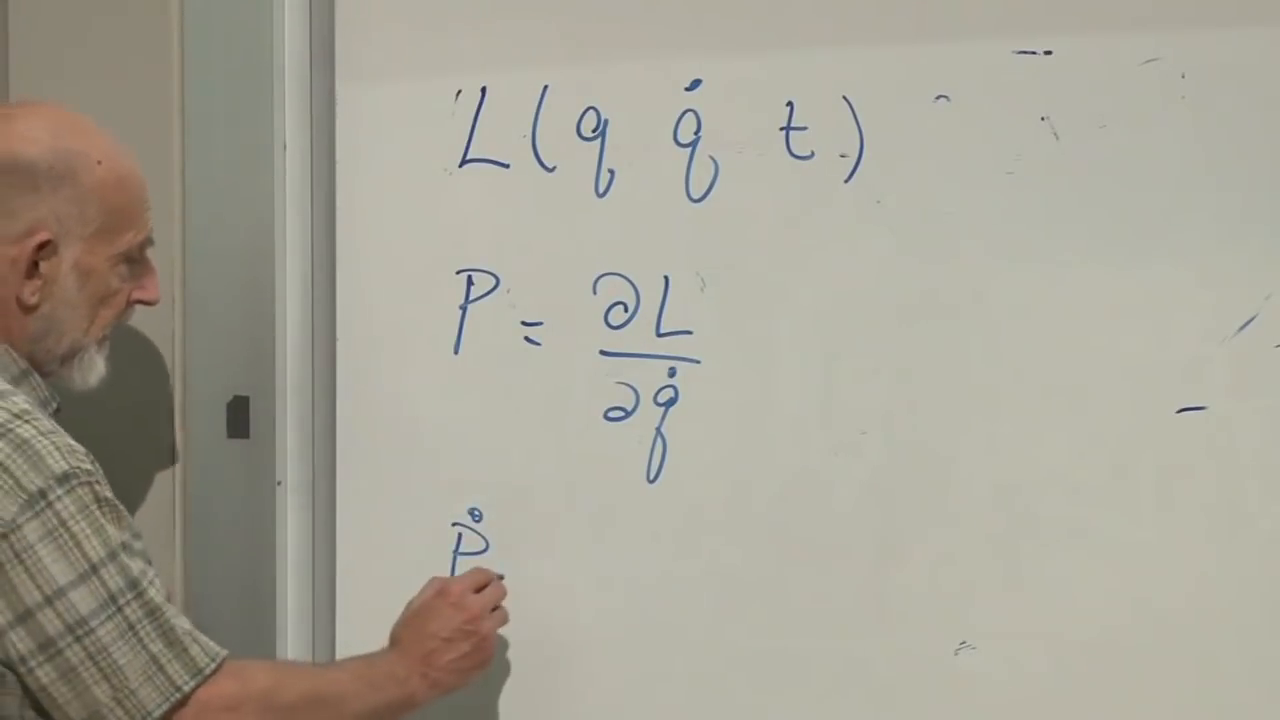
\includegraphics[width=0.66\textwidth]{lecture_05_figure_03.png}\caption{Die Zusammenfassung an der Tafel beginnt mit \(L(q,\dot q,t)\), dem kanonischen Impuls und der Euler---Lagrange-Gleichung.}\lectureframe{01:31:37}\end{figure}

Diese Formeln umfassen eine Definition, Bewegungsgleichungen, die Ladung einer gewöhnlichen kontinuierlichen Symmetrie und die Ladung der Zeittranslation. Es gibt nur wenige Kniffe; entscheidend ist, die Formeln herleiten zu können, statt voneinander losgelöste Ausdrücke auswendig zu lernen.

\section{Wozu dient die Lagrange- oder Hamilton-Mechanik?}

\begin{classroomqa}\audiencequestion{Lässt sich die Mechanik gleichwertig mit \(L\) oder \(H\) beschreiben, und warum entscheidet man sich für die eine oder andere Formulierung?\lecturetimestamp{01:37:16--01:39:18}}\lecturerresponse{Bei regulärer Legendre-Transformation sind sie äquivalent, doch sie heben unterschiedliche Strukturen hervor. Die Lagrange-Mechanik geht auf natürliche Weise von stationärer Wirkung aus. Die Hamilton-Mechanik ist zunächst abstrakter, doch ihre Gleichungen sind einfach, und sie wird in der Quantenmechanik zentral. Der Hamiltonian ist die Energie, seine Bedeutung geht aber weit über das Energieerhaltungsgesetz hinaus.}\end{classroomqa}

\begin{classroomqa}\audiencequestion{Kannte Newton die Hamiltonsche Form der Energieerhaltung?\lecturetimestamp{01:39:29--01:39:56}}\lecturerresponse{Soweit aus den historischen Quellen hervorgeht, nicht in dieser Formulierung. Newtons ausdrücklich angegebener Rahmen war das Kraftgesetz \(F=ma\).}\end{classroomqa}

\begin{classroomqa}\audiencequestion{Warum sollte jedes physikalische System eine Lagrangefunktion besitzen? Ist das lediglich eine experimentelle Tatsache?\lecturetimestamp{01:39:57--01:42:37}}\lecturerresponse{Für die hier betrachteten abgeschlossenen Systeme ist es eine empirische Tatsache und folgt außerdem aus der tiefer liegenden Quantenbeschreibung. Mathematisch konsistente Differentialgleichungen lassen sich angeben, die keine Euler---Lagrange-Gleichungen sind. Zum Beispiel ist \(\dot x=-x\) problemlos lösbar, doch als fundamentales Gesetz für ein abgeschlossenes System mit einer Koordinate hat es den informationsvernichtenden Charakter einer Dissipation. Die klassische Mechanik geht der Quantenmechanik logisch nicht voraus; ihre fundamentale Struktur ist von der Quantenmechanik übernommen. Der genaue Grund muss noch warten.}\end{classroomqa}

\begin{classroomqa}\audiencequestion{Wenn jedes reale abgeschlossene System eine Lagrangefunktion hat, entspricht dann jede Funktion, die wir Lagrangefunktion nennen, einem in der Natur vorkommenden System?\lecturetimestamp{01:42:39--01:42:54}}\lecturerresponse{Nein. Der formale Kalkül lässt viele Funktionen zu, die durch kein bekanntes physikalisches System verwirklicht werden.}\end{classroomqa}

\begin{classroomqa}\audiencequestion{Ist die Lagrangefunktion vor allem ein Werkzeug, um Potentiale zu erfinden?\lecturetimestamp{01:42:54--01:43:32}}\lecturerresponse{Sie ist vielseitiger. Mit ihr lassen sich mögliche mechanische Systeme ordnen; außerdem ist sie häufig der kürzeste praktikable Weg zu den Bewegungsgleichungen.}\end{classroomqa}

Das Doppelpendel veranschaulicht diesen praktischen Vorteil. Wählen wir zwei Winkel, berechnen wir die Geschwindigkeiten beider Massen anhand dieser Winkel und ihrer Zeitableitungen, bilden wir \(T-V\) und überlassen die implizite Berücksichtigung der Zwangskräfte den Euler---Lagrange-Gleichungen. Das ist deutlich übersichtlicher, als sämtliche Spannkräfte und Beschleunigungen mit \(F=ma\) zu bestimmen.

\begin{figure}[htbp]\centering
  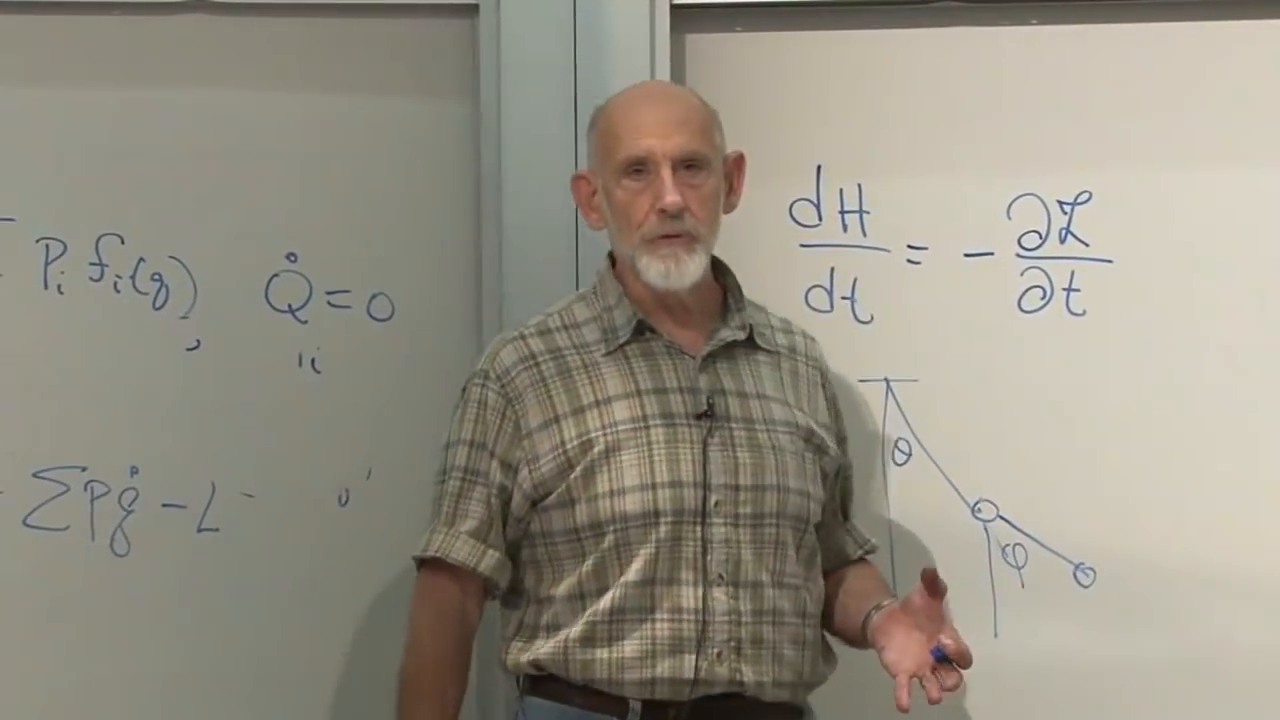
\includegraphics[width=0.84\textwidth]{lecture_05_figure_05.png}\caption{Die Identität für die Änderungsrate der Energie bleibt neben der Skizze des Doppelpendels an der Tafel stehen.}\lectureframe{01:45:39}\end{figure}

\begin{figure}[htbp]\centering
  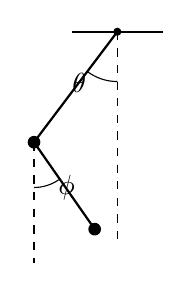
\begin{tikzpicture}[scale=1.15]
    \draw[thick] (-0.5,0) -- (0.5,0);
    \fill (0,0) circle (0.045);
    \draw[dashed] (0,0) -- (0,-2.3);
    \draw[thick] (0,0) -- (-0.92,-1.22);
    \fill (-0.92,-1.22) circle (0.07);
    \draw[dashed] (-0.92,-1.22) -- (-0.92,-2.55);
    \draw[thick] (-0.92,-1.22) -- (-0.25,-2.18);
    \fill (-0.25,-2.18) circle (0.07);
    \draw (0,-0.55) arc (-90:-127:0.55);
    \node at (-0.42,-0.56) {$\theta$};
    \draw (-0.92,-1.72) arc (-90:-55:0.48);
    \node at (-0.56,-1.72) {$\phi$};
  \end{tikzpicture}\caption{Verallgemeinerte Winkelkoordinaten für ein Doppelpendel.}\end{figure}

Auch ein Variablenwechsel ist effizient: Man transformiert eine Lagrangefunktion und leitet anschließend ihre Bewegungsgleichungen her, statt jede Kraftgleichung einzeln zu transformieren.

\begin{classroomqa}
  \audiencequestion{Ist das Doppelpendel im Wesentlichen ein weiteres Dreikörpersystem, etwa Sonne, Erde und Mond, bei dem ein Körper als Bezugspunkt behandelt wird?
  \lecturetimestamp{01:45:06--01:45:25}}
  \lecturerresponse{Diese Analogie erfasst die Hierarchie, auch wenn die Stäbe andere Zwangsbedingungen auferlegen. In beiden Fällen kann man in einer Näherung einen sehr massereichen oder festgehaltenen Bestandteil als Bezugsstruktur behandeln.}
\end{classroomqa}

\begin{classroomqa}
  \audiencequestion{Beim Doppelpendel verwendet man \(T-V\), obwohl gerade allgemeinere Lagrangefunktionen behandelt wurden. Wann ist \(T-V\) gültig?
  \lecturetimestamp{01:46:08--01:46:58}}
  \lecturerresponse{Für gewöhnliche nichtrelativistische Teilchen in einem Inertialsystem, bei denen keine magnetische Geschwindigkeitskopplung vorliegt, gilt die bekannte Form. Rotierende Bezugssysteme, relativistische Systeme und Magnetfelder erfordern allgemeinere Terme.}
\end{classroomqa}

\begin{classroomqa}
  \audiencequestion{Liegen Stöße außerhalb dieser Beschreibung?
  \lecturetimestamp{01:47:00--01:48:05}}
  \lecturerresponse{Elastische Stöße entstehen durch kurzreichweitige Kräfte und damit durch Potenziale. Inelastische Stöße sind auf mikroskopischer Ebene weiterhin mechanisch, doch Energie geht in innere Schwingungen, Verformung und Wärme über. Eine Beschreibung des Schwerpunkts, die diese Freiheitsgrade auslässt, ist unvollständig.}
\end{classroomqa}

\begin{classroomqa}
  \audiencequestion{Lässt sich ein Baseball, der von einem Schläger getroffen wird, mit \(F=ma\) analysieren?
  \lecturetimestamp{01:48:05--01:48:33}}
  \lecturerresponse{Nur in einer groben Beschreibung. Eine vollständige Behandlung muss Verformung, Erwärmung, mögliche Schäden am Ball und vielleicht auch einen zerbrechenden Schläger berücksichtigen. Diese inneren Freiheitsgrade machen einen realistischen Aufprall viel schwieriger als einen Stoß von Punktteilchen.}
\end{classroomqa}

\begin{classroomqa}
  \audiencequestion{Wie steht es mit einem ausgedehnten starren Körper?
  \lecturetimestamp{01:48:34--01:49:00}}
  \lecturerresponse{Starre Körper lassen sich entweder mit Newtonschen Methoden oder mit einer \(T-V\)-Lagrangefunktion untersuchen, die in Translations- und Rotationskoordinaten geschrieben ist. Diese Lagrangefunktion aufzustellen, ist eine nützliche Übung.}
\end{classroomqa}

\begin{classroomqa}
  \audiencequestion{Bedeutet die quantenmechanische Energie--Zeit-Unschärferelation, dass die Energie nicht streng erhalten ist?
  \lecturetimestamp{01:49:01--01:49:29}}
  \lecturerresponse{Nein. Die Energie kann streng erhalten sein. Die Relation besagt, dass eine hochgenaue Bestimmung der Energie eine lange Beobachtungszeit erfordert; sie ersetzt nicht den Erhaltungssatz.}
\end{classroomqa}

\begin{classroomqa}
  \audiencequestion{Sind Newtonsche und Lagrangesche Mechanik logisch gleichwertig?
  \lecturetimestamp{01:49:36--01:50:07}}
  \lecturerresponse{Sie sind in dem üblichen Gültigkeitsbereich, in dem beide Formulierungen anwendbar sind, gleichwertig. Man kann dennoch Lagrangefunktionen konstruieren, deren Bewegungsgleichungen nicht der elementaren Form \(m\ddot x=F(x)\) ähneln.}
\end{classroomqa}

\section{Ein koordinatenabhängiger kinetischer Term}

Betrachten wir das bewusst ungewohnte Beispiel
\begin{equation}
  L=\frac12q^2\dot q^2-\frac12q^2.
  \label{eq:l5-nonstandard-l}
\end{equation}
Es ist eine gültige Lagrangefunktion mit einem koordinatenabhängigen Koeffizienten des kinetischen Terms. Man kann auch Terme betrachten, die linear in der Geschwindigkeit sind, etwa \(q\dot q\); in diesem eindimensionalen Beispiel ist gerade dieser Term jedoch eine totale Ableitung und würde die Bewegungsgleichungen nicht verändern.

Der kanonische Impuls ist
\begin{equation}
  p=\frac{\partial L}{\partial\dot q}=q^2\dot q,
  \label{eq:l5-nonstandard-p}
\end{equation}
also gilt
\begin{equation}
  \dot p=q^2\ddot q+2q\dot q^2,
  \qquad
  \frac{\partial L}{\partial q}=q\dot q^2-q.
  \label{eq:l5-nonstandard-derivatives}
\end{equation}
Damit lautet die Bewegungsgleichung
\begin{equation}
  q^2\ddot q+q\dot q^2=-q.
  \label{eq:l5-nonstandard-eom}
\end{equation}

\begin{figure}[htbp]
  \centering
  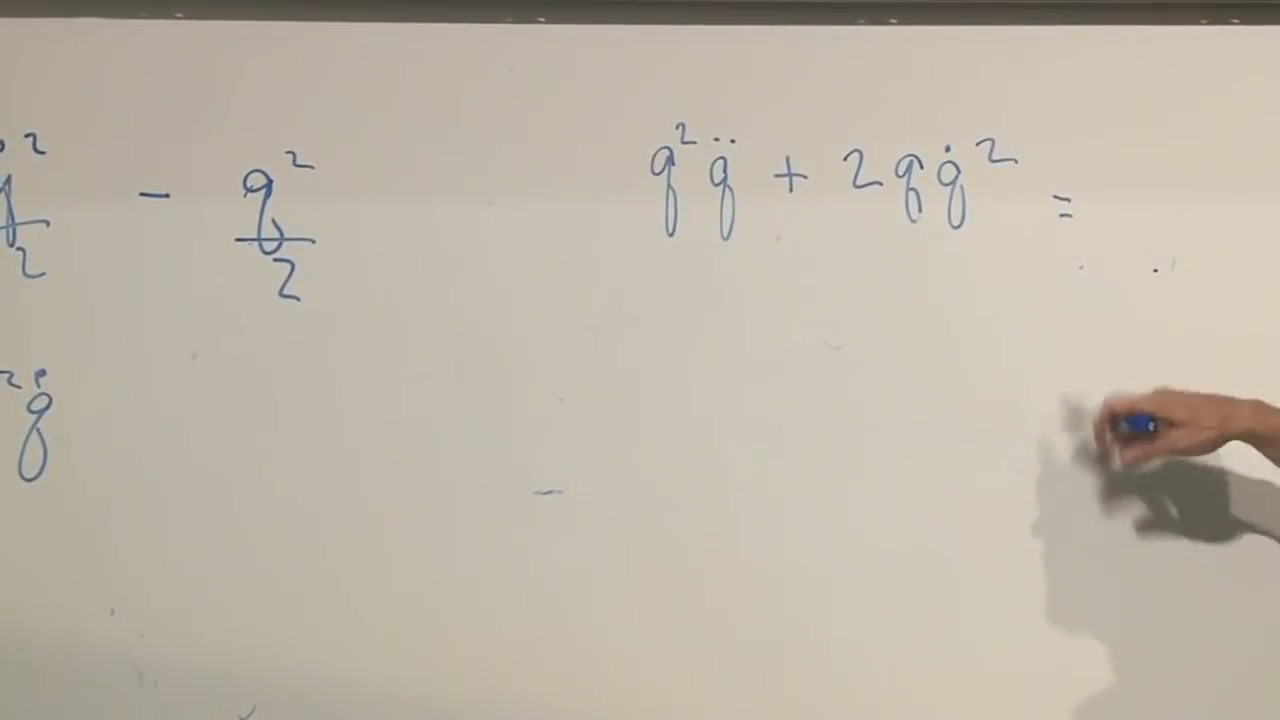
\includegraphics[width=0.80\textwidth]{lecture_05_figure_06.png}
  \caption{Die abgeleitete Impulsgröße im Beispiel mit koordinatenabhängigem kinetischem Term.}
  \lectureframe{01:52:32}
\end{figure}

\begin{classroomqa}
  \audiencequestion{Kann man die Gleichung durch \(q\) teilen?
  \lecturetimestamp{01:53:22--01:53:39}}
  \lecturerresponse{Nur dort, wo \(q\neq0\) gilt. Bei \(q=0\) sind der Koeffizient des kinetischen Terms und die Legendre-Abbildung entartet; durch Division würde man daher einen singulären Punkt ausschließen, der gesondert behandelt werden muss.}
\end{classroomqa}

Die Hamiltonfunktion lautet
\begin{align}
  H&=p\dot q-L
  \notag\\
   &=q^2\dot q^2-
     \left(\frac12q^2\dot q^2-\frac12q^2\right)
  \notag\\
   &=\frac12q^2\dot q^2+\frac12q^2.
  \label{eq:l5-nonstandard-h}
\end{align}

\begin{classroomqa}
  \audiencequestion{Kann \(q^2\dot q^2/2\) weiterhin als kinetische Energie bezeichnet werden?
  \lecturetimestamp{01:54:41--01:55:07}}
  \lecturerresponse{Ja. In diesem ausgearbeiteten Beispiel hat die Hamiltonfunktion wieder die Form eines positiven kinetischen Terms plus eines Potenzialterms. Entscheidend ist, dass die formalen Definitionen auch ohne vorherige Annahme der elementaren Form mit konstanter Masse funktionieren.}
\end{classroomqa}

\section{Dissipation und der tiefere Ursprung des Formalismus}

\begin{classroomqa}
  \audiencequestion{Wie wird Reibung in eine Lagrangefunktion aufgenommen?
  \lecturetimestamp{01:55:09--01:56:17}}
  \lecturerresponse{In dem hier betrachteten einfachen, abgeschlossenen System mit endlich vielen Freiheitsgraden nicht als fundamentale Kraft. Makroskopische Reibung ist ein statistischer Effekt, der aus einer enormen Zahl mikroskopischer Freiheitsgrade hervorgeht. Die Atome gehorchen weiterhin der zugrunde liegenden Mechanik, doch eine reduzierte Beschreibung, die sie nicht verfolgt, zeigt Dissipation.}
\end{classroomqa}

\begin{classroomqa}
  \audiencequestion{Wie gelangte Hamilton zu seiner Formulierung?
  \lecturetimestamp{01:56:22--01:56:37}}
  \lecturerresponse{Hier wurde keine historische Herleitung gegeben. Für den vorliegenden Kurs ist vor allem wichtig zu verstehen, wie die Formulierung funktioniert.}
\end{classroomqa}

\begin{classroomqa}
  \audiencequestion{Gibt es ein allgemeineres Verfahren, um eine Lagrangefunktion zu finden, wenn sie nicht offensichtlich die Form \(T-V\) hat?
  \lecturetimestamp{01:56:43--01:58:54}}
  \lecturerresponse{Experimente, eine begründete Vermutung, ein Symmetrieprinzip oder die Rekonstruktion aus gewünschten Gleichungen können die Funktion liefern. Die Analysis selbst zu fragen, woher ihre Eingabe kommt, ist so, als fragte man die Definition einer Ableitung, woher \(f(x)\) stammt. Die Analysis sagt uns, was zu tun ist, sobald die Funktion festgelegt ist. Warum die abgeschlossenen Systeme der Natur dieser abstrakten Struktur entsprechen, beantwortet die Quantenmechanik auf einer tieferen Ebene.}
\end{classroomqa}

Dieser Punkt knüpft an die einleitenden Themen des Kurses an. Die fundamentale Hamiltonsche Zeitentwicklung ist deterministisch und umkehrbar, insofern sich Trajektorien nicht vereinigen und Information nicht einfach vernichtet wird. Der Zusammenhang zwischen dieser Eigenschaft und der Phasenraumformulierung wird schrittweise entwickelt.

\begin{classroomqa}
  \audiencequestion{Ist die Variationsrechnung lediglich rückwärts von den gewünschten klassischen Gleichungen ausgegangen, und erhält die Quantenmechanik ihre Lagrangefunktion auf dieselbe Weise?
  \lecturetimestamp{01:59:37--02:01:07}}
  \lecturerresponse{Bei der elementaren klassischen Konstruktion kann man tatsächlich eine Wirkung wählen, deren stationäre Wege die bekannten Gleichungen ergeben. In der Quantenmechanik ist die logische Reihenfolge eine andere: Sie geht auf natürliche Weise von der Hamiltonfunktion aus und kann zu einer Lagrangebeschreibung gelangen. Dort ist die Hamiltonfunktion anschaulicher, obwohl sie in der klassischen Mechanik zunächst abstrakt erscheint.}
\end{classroomqa}

\begin{classroomqa}
  \audiencequestion{Kann die Quantenmechanik Reibung beschreiben?
  \lecturetimestamp{02:01:08--02:02:05}}
  \lecturerresponse{Ja, aber eine fundamentale Beschreibung muss die Freiheitsgrade der Umgebung einschließen. Ein Teilchen, das sich durch eine viskose Flüssigkeit bewegt, lässt sich nicht vollständig beschreiben, ohne auch die Teilchen der Flüssigkeit einzubeziehen. Reibung ist der komplizierte kollektive Effekt, der entsteht, wenn diese Freiheitsgrade nicht einzeln verfolgt werden.}
\end{classroomqa}
